\documentclass[10pt]{article}
\usepackage[margin=0.60in]{geometry}
\usepackage{booktabs,enumitem,fancyhdr,graphicx,listings,tabularx,titlesec,xcolor}
\usepackage[hidelinks]{hyperref}
\graphicspath{{docs/lessons/assets/}{../assets/}}
\hypersetup{
 pdftitle={ADK Lesson 058: Nonblocking Multiplexed Digits},
 pdfauthor={Kevin Shanahan},
 pdfsubject={Supplied-time four-digit formatting, ordered refresh intent, refresh-loss evidence, and deterministic E0 replay},
 pdflang={en-US}}
\pagestyle{fancy}\fancyhf{}
\lhead{\textsc{ADK Lesson 058}}\rhead{Nonblocking Multiplexed Digits}
\cfoot{\thepage}\setlength{\headheight}{14pt}
\setlength{\parindent}{0pt}\setlength{\parskip}{3pt}
\setlist{nosep,leftmargin=1.45em}
\titleformat{\section}{\Large\bfseries}{\thesection}{0.5em}{}
\newcommand{\lessonbox}[1]{\begin{center}\fbox{\parbox{0.92\linewidth}{#1}}\end{center}}
\newcommand{\blankline}{\rule{0.76in}{0.4pt}}
\newcommand{\longblank}{\rule{1.28in}{0.4pt}}
\lstset{
 basicstyle=\ttfamily\footnotesize,
 columns=fullflexible,
 breaklines=true,
 frame=single,
 rulecolor=\color{black},
 showstringspaces=false}

\begin{document}
\small
\begin{center}
 {\Huge\bfseries Nonblocking Multiplexed Digits}\\[3pt]
 {\Large Make ghost-prevention order and missed service visible}\\[7pt]
 \fbox{\textbf{E0 COPIED POLICY REPLAY --- ZERO DISPLAY HARDWARE}}
\end{center}
\begin{tabularx}{\linewidth}{@{}>{\bfseries}l X >{\bfseries}l X@{}}
Lesson & 058 --- component & Time & 120--180 minutes\\
Prerequisite & Lesson 010 glyph vocabulary & Board & compile-only Mega replay\\
Capacity & four logical cells & Observation & named memory result cells\\
\end{tabularx}

\lessonbox{\textbf{Responsibility.}
\texttt{MultiplexedDigitPolicy} formats one copied value into four logical
glyph cells and emits one bounded, ordered refresh transaction when supplied
time says service is due. It owns no pin, timer, interrupt, digit driver,
display, resistor, supply, or powered circuit.}

\section{Begin with the illusion}
A four-digit display can appear steady even though a controller selects only
one digit at a time. The illusion depends on repeated service and on changing
the shared segment lines only while every digit select is inactive. Lesson 058
models that ordering as copied intent. It does not claim that any LED lit.

\begin{center}
% ADK visual: pencil
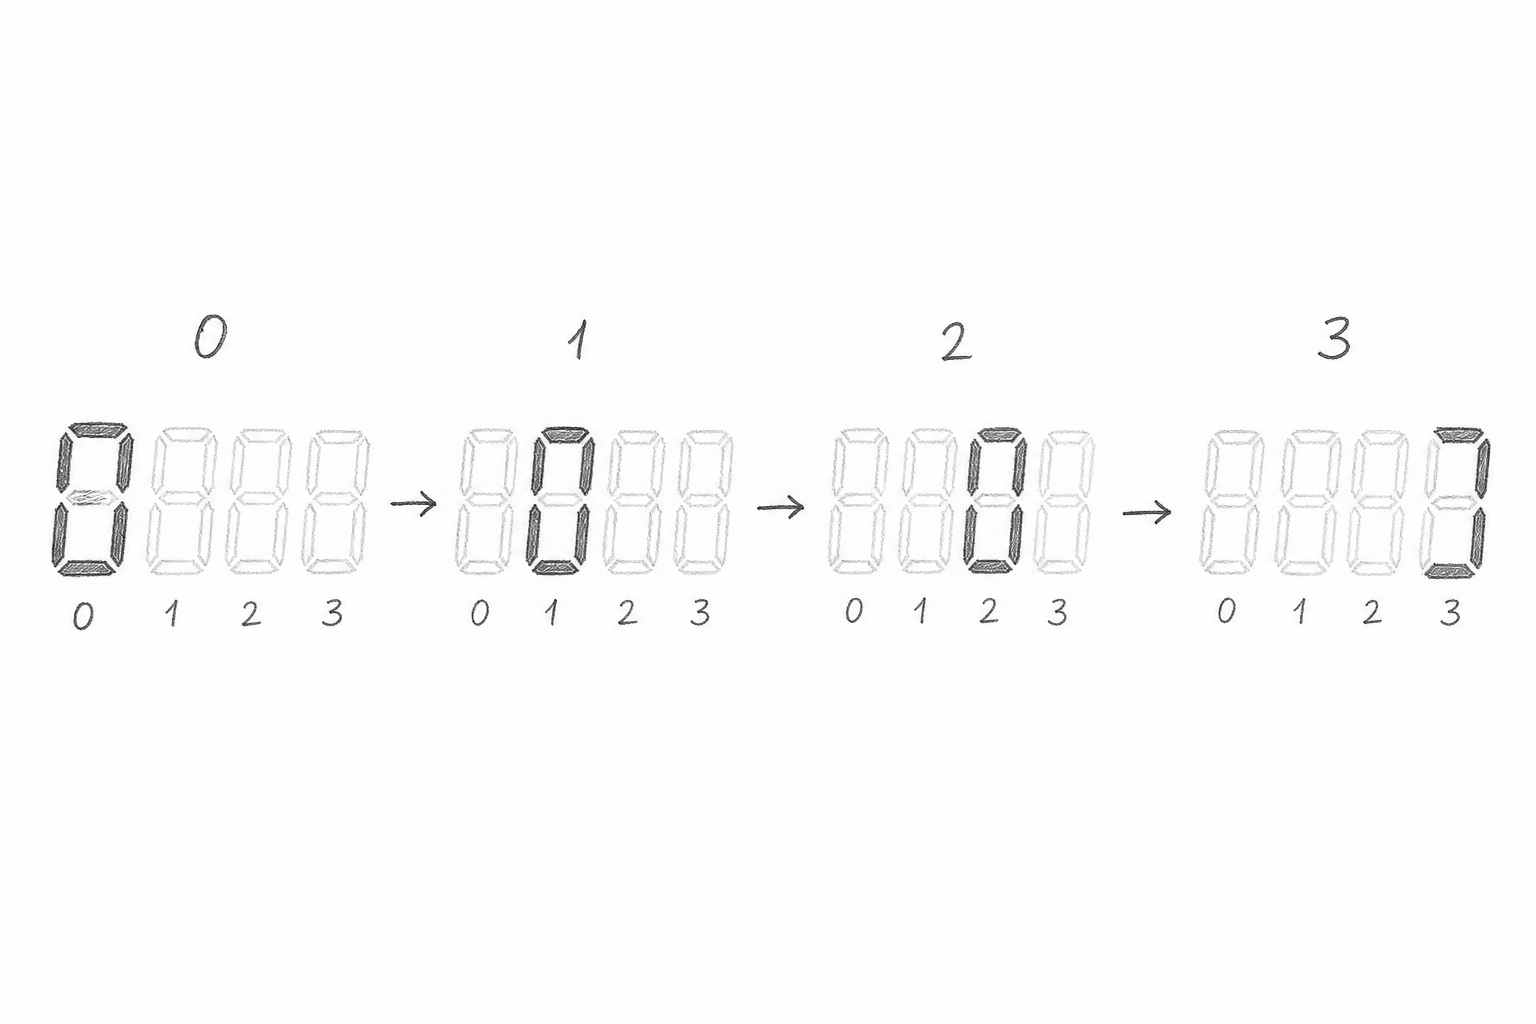
\includegraphics[width=0.94\linewidth,height=2.05in,keepaspectratio]
 {058-scanbook-pencil.png}

\small\textit{Alternative text: a rough pencil flipbook shows exactly one
selected digit moving through zero-based phases 0, 1, 2, and 3 from left to
right.}
\end{center}

The drawing is a timing mnemonic, not a breadboard layout or formal electrical
schematic. At E0, the observation place is the canonical sketch's copied
transaction cells.

\section{Keep formatting exact}
The display has four cells numbered left to right from zero through three.
Each cell carries the canonical Lesson 010 segments \(a,b,c,d,e,f,g,dp\).
Values from 0 through 9,999 render as decimal digits. Larger values render
four dashes, clear every decimal point, and report overflow; they never wrap
or truncate.

Leading zeros may be shown or blanked, but the value zero always retains one
zero. Decimal-mask bit zero names the rightmost cell. Segment polarity and
digit-select polarity are separate configuration values. A common-anode or
common-cathode label does not reveal the topology of a future digit driver.

\begin{tabularx}{\linewidth}{@{}l l l X@{}}
\toprule
Input & Leading-zero policy & Decimal mask & Predict the four cells\\
\midrule
0 & blank & \texttt{0x00} & blank, blank, blank, zero\\
42 & blank & \texttt{0x02} & blank, blank, four, two with decimal\\
42 & show & \texttt{0x02} & zero, zero, four, two with decimal\\
9999 & either & \texttt{0x0A} & four digits with requested decimal points\\
10000 & either & any & four dashes; no decimal points\\
\bottomrule
\end{tabularx}

\section{Prove the three-stage transaction}
Each due \texttt{refresh(now)} call emits exactly one transaction. First,
every digit select is inactive while the prior segment levels remain. Second,
every select remains inactive while the next segment levels appear. Third,
exactly one digit select becomes active. The order is part of the public
evidence because a final mask alone would conceal a ghost-producing update.

\begin{center}
% ADK visual: pencil
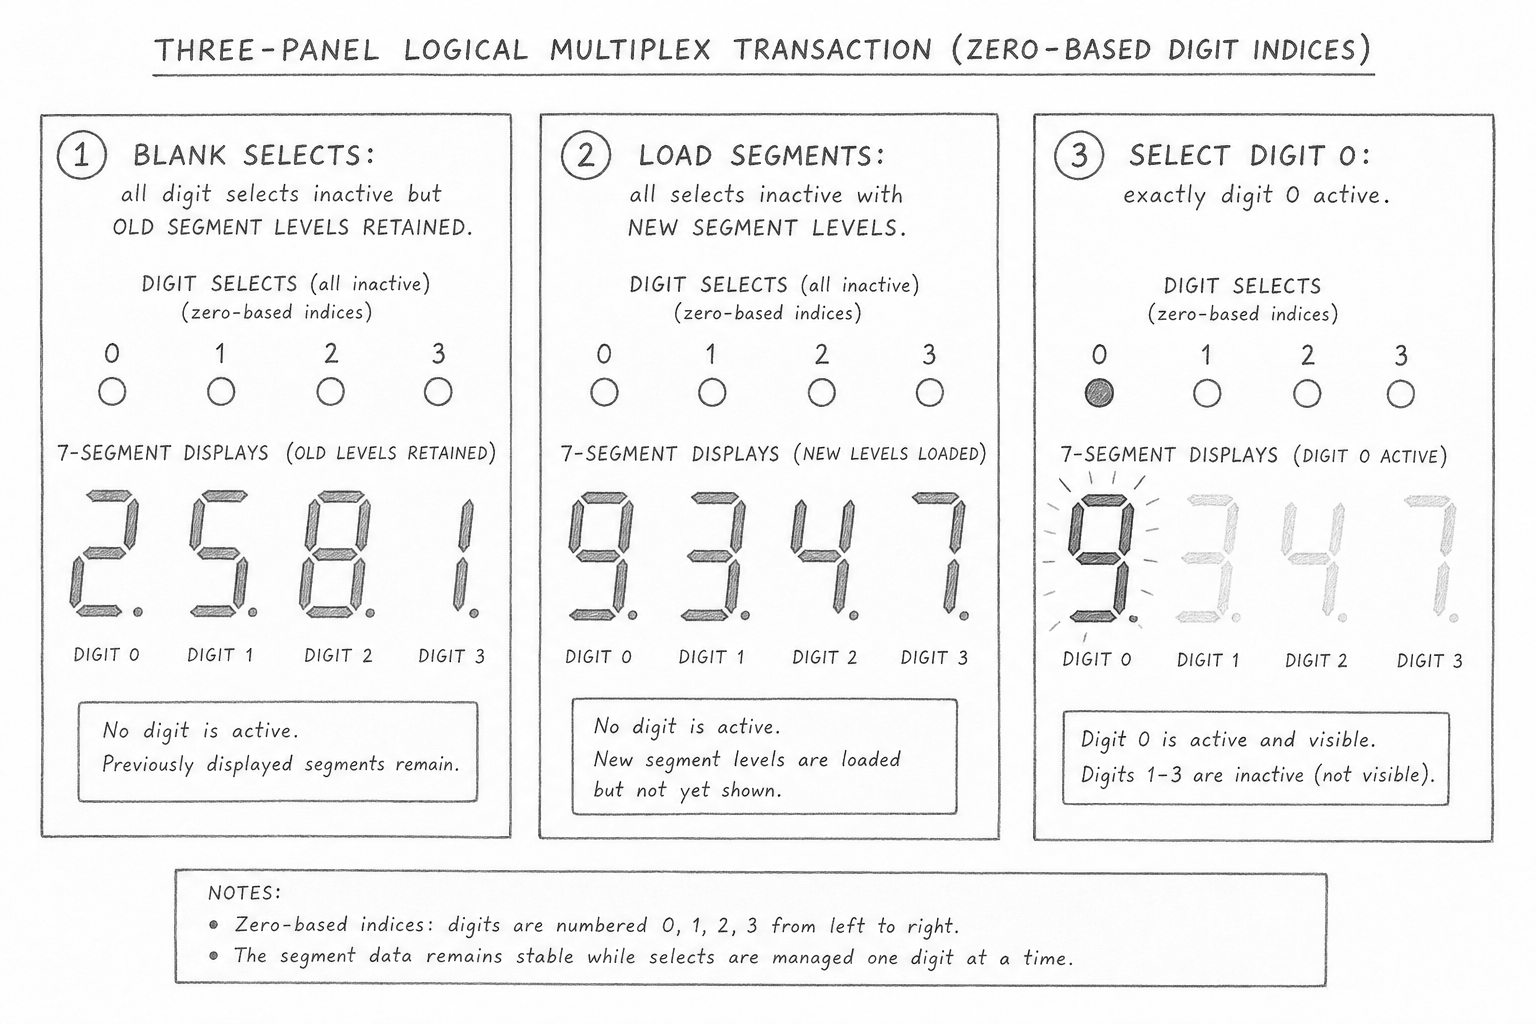
\includegraphics[width=0.95\linewidth,height=2.15in,keepaspectratio]
 {058-three-stage-refresh-pencil.png}

\small\textit{Alternative text: three hand-drawn frames labeled blank,
segments, and select show all digit selects inactive, then the next segment
mask, then exactly one selected digit. Pencil arrows enforce the order.}
\end{center}

\begin{tabularx}{\linewidth}{@{}l X X@{}}
\toprule
Stage & Predict & Inspect in copied evidence\\
\midrule
blank & all selects inactive; old segment levels retained &
\texttt{stages[0]} select and segment masks\\
segments & all selects inactive; next segment levels applied &
\texttt{stages[1]} select and segment masks\\
select & one and only one digit active &
\texttt{stages[2]} selected index and masks\\
\bottomrule
\end{tabularx}

\section{Service one phase, never catch up}
The default service period is 1 ms. Calls before the period emit nothing. A
due call advances exactly one digit and reanchors to the supplied
\texttt{now}. It never loops to replay missed phases. Initialization has one
explicit exception: its first refresh at the initialization timestamp emits
digit zero's complete transaction.

The maximum accepted gap is 4 ms. Equality remains valid; the next tick
latches \texttt{RefreshLost}, publishes blank intent, and requires explicit
reset. Equal timestamps are idempotent after first service. Backward time and
an exact unsigned half-range difference reject atomically.

\begin{center}
% ADK visual: pencil
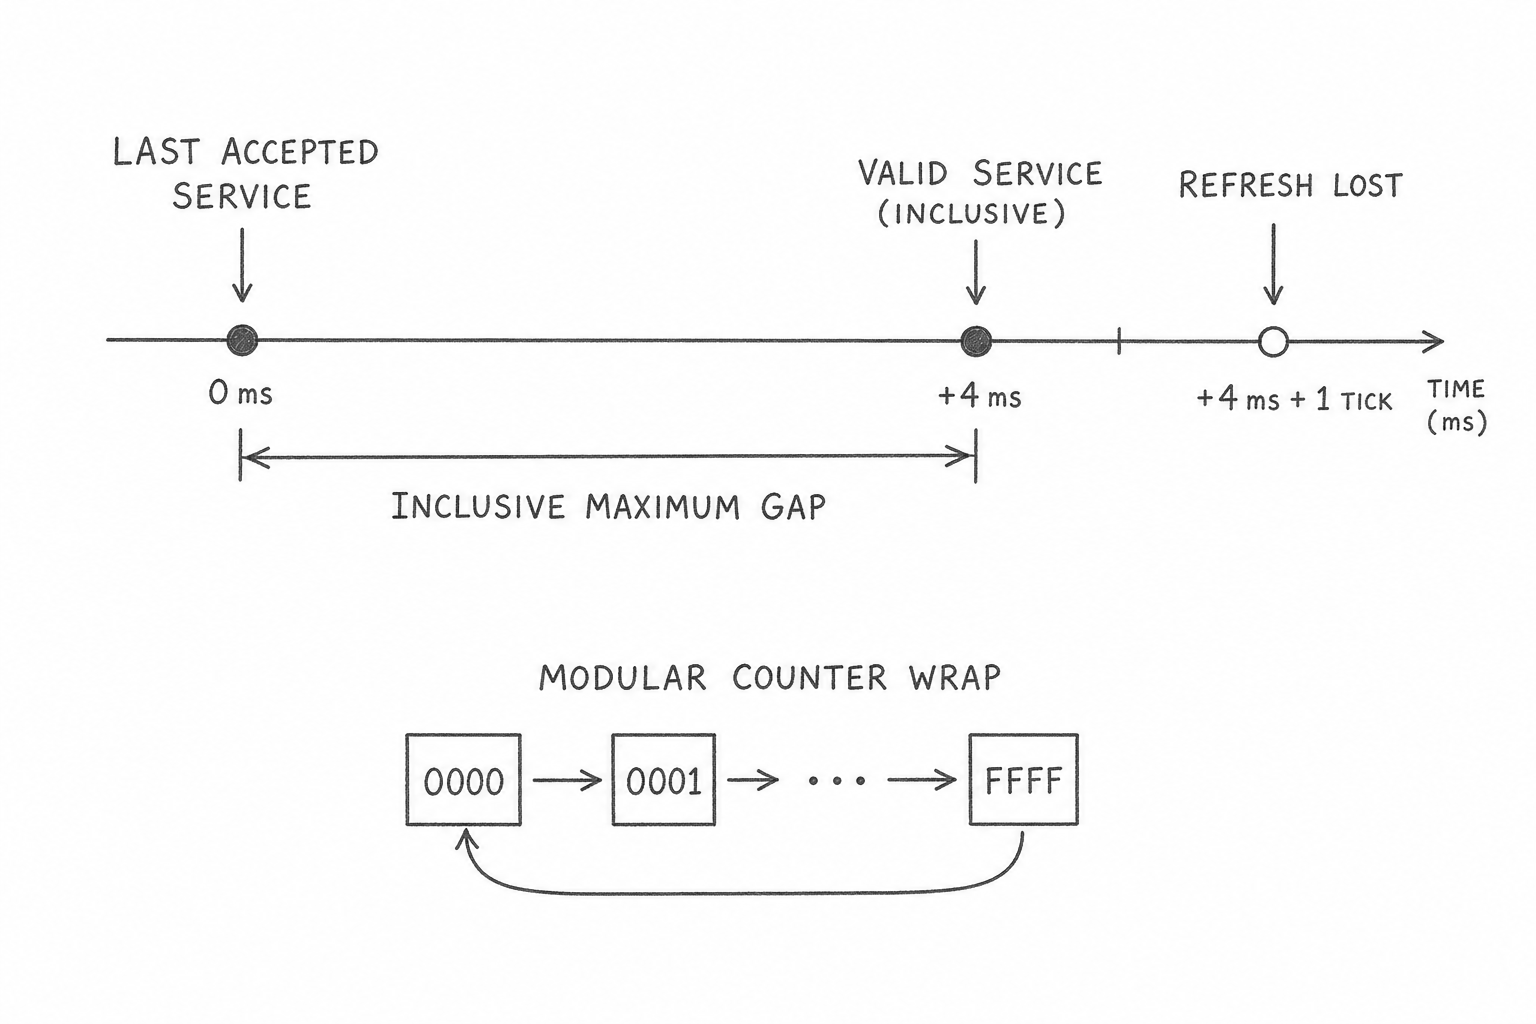
\includegraphics[width=0.96\linewidth,height=1.75in,keepaspectratio]
 {058-refresh-deadline-pencil.png}

\small\textit{Alternative text: a pencil timeline spans the full interval
from the last accepted service to the inclusive four-millisecond boundary;
the next tick is separately labeled refresh lost, with modular wrap below.}
\end{center}

\begin{tabularx}{\linewidth}{@{}l l l X@{}}
\toprule
Supplied time & Prior accepted time & Prediction & Reason\\
\midrule
1000 & initialized at 1000 & digit zero transaction & first-service exception\\
1000 & accepted at 1000 & no transaction & equal-time idempotence\\
1999 & accepted at 1000 & no transaction & one tick early\\
2000 & accepted at 1000 & one transaction & service period reached\\
6000 & accepted at 2000 & one transaction & inclusive maximum gap\\
6001 & accepted at 2000 & blank, \texttt{RefreshLost} & first invalid gap\\
\bottomrule
\end{tabularx}

\newpage
\section{Publish a frame without tearing}
Formatting uses \texttt{preview()}, \texttt{canCommit()}, and
\texttt{commit()}. A preview is bound to its owner, lifecycle, configuration,
and base generation. Foreign, stale, altered, or consumed previews cannot
commit.

A successful commit changes the desired glyph bank, not the bank currently
being scanned. The desired bank becomes active only at the next digit-zero
boundary. Each bank retains a local generation and the caller-supplied source
snapshot sequence.

\begin{center}
% ADK visual: pencil
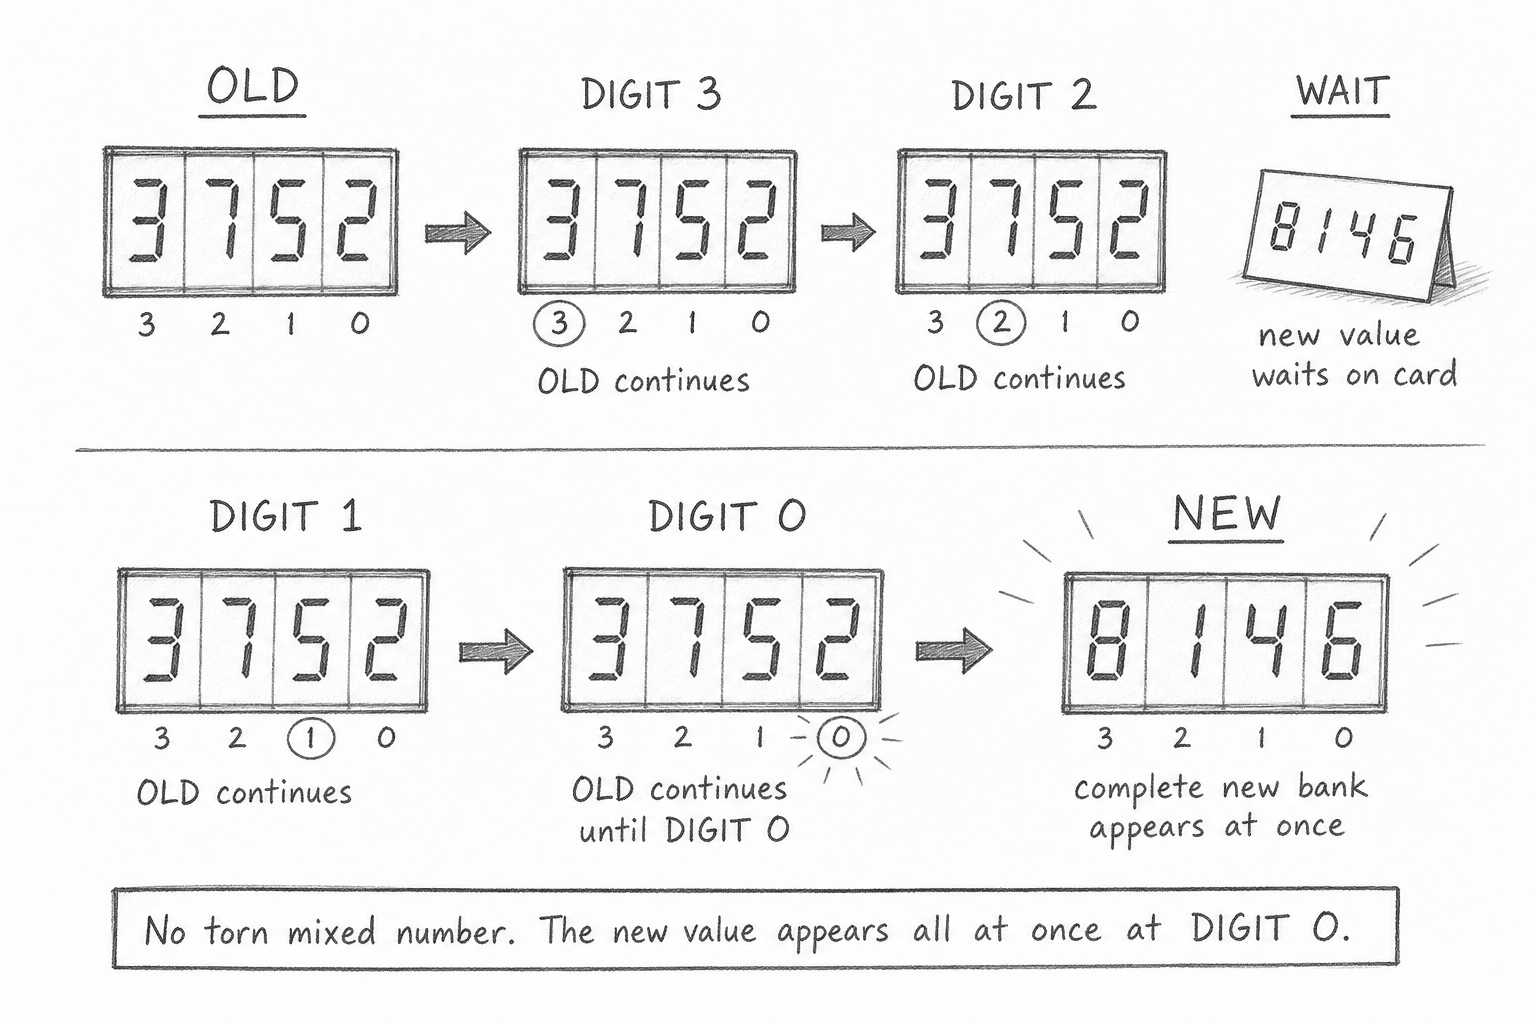
\includegraphics[width=0.94\linewidth,height=2.05in,keepaspectratio]
 {058-frame-swap-pencil.png}

\small\textit{Alternative text: a hand-drawn current-frame card continues
through digits two and three while a desired-frame card waits behind a gate;
at digit zero, the complete desired card replaces the complete current card.}
\end{center}

Construction is inert. \texttt{reset(now)} preserves immutable
configuration, invalidates previews, clears the frame, and returns to the
initialized blank and digit-zero-armed state. \texttt{shutdown()} invalidates
previews and is idempotent; service remains inert until later initialization.
The policy retains no caller pointer, reads no clock, allocates nothing,
recurses nowhere, invokes no callback, and performs bounded work.

\section{Read the canonical replay}
The canonical compile-only Mega sketch follows acquire, configure, start and
then observe, decide, actuate. Its ``actuation'' is assignment to named
volatile result cells:

\begin{lstlisting}[language=C++]
MultiplexedDigitPreview candidate;
const Status previewStatus =
    display.preview(value, showLeadingZeros,
                    decimalMask, sourceSequence,
                    candidate);
const Status commitStatus = previewStatus.ok()
    ? display.commit(candidate) : previewStatus;
const Result<MultiplexedDigitTransaction> result =
    display.refresh(now);
\end{lstlisting}

The exact source is downloadable as text. Do not credit Serial output. A host
test may compare every field of a copied transaction; the sketch offers the
same logical evidence through inspectable memory cells.

\section{Run predict, observe, interpret}
\begin{enumerate}
 \item \textbf{Initialize.} Predict blank intent, digit zero armed, and no
       hardware claims. Observe lifecycle, blank, and generation cells.
       Interpret success as E0 policy initialization only.
 \item \textbf{First refresh.} Predict blank/segments/select order at the
       initialization timestamp. Observe all three copied stage cells.
       Interpret their order; do not infer a waveform.
 \item \textbf{Format.} Predict the complete bank for zero, 42 with and
       without leading zeros, 9,999, and overflow. Observe desired glyphs,
       decimal mask, overflow, source sequence, and generation.
 \item \textbf{Swap.} Commit while digit three is active. Predict that the old
       bank finishes and the new bank appears only at digit zero. Observe
       desired and active generations at each service.
 \item \textbf{Timing.} Exercise early, due, equal, wraparound, exact 4 ms,
       and one-tick-late calls. Observe disposition, phase, and blank intent.
 \item \textbf{Recover.} Predict that refresh loss remains latched until
       reset. Observe inert service before reset, then blank and armed state.
 \item \textbf{Shutdown.} Predict no later transaction. Observe lifecycle and
       copied blank intent. Interpret no physical blanking claim.
\end{enumerate}

\begin{tabularx}{\linewidth}{@{}l l l l X@{}}
\toprule
Case & time & active generation & digit & result / interpretation\\
\midrule
first service & \blankline & \blankline & \blankline & \longblank\\[7pt]
early & \blankline & \blankline & \blankline & \longblank\\[7pt]
digit-zero swap & \blankline & \blankline & \blankline & \longblank\\[7pt]
exact gap limit & \blankline & \blankline & \blankline & \longblank\\[7pt]
one tick late & \blankline & \blankline & \blankline & \longblank\\
\bottomrule
\end{tabularx}

\section{Diagnose from the first violated contract}
\begin{center}
% ADK visual: pencil
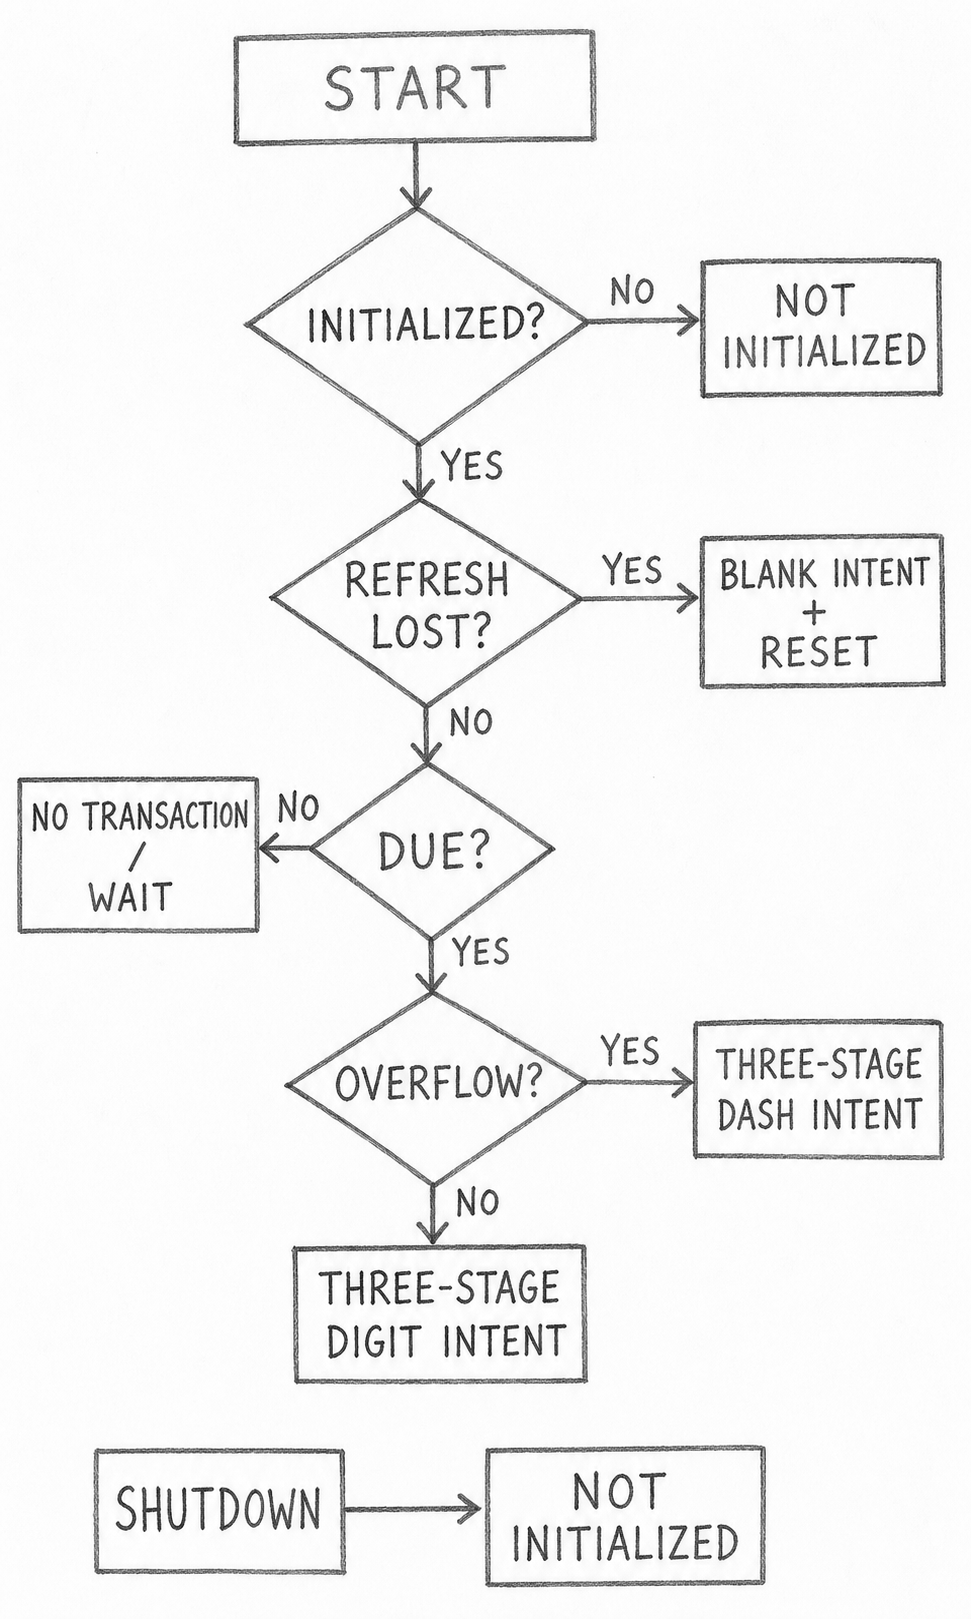
\includegraphics[width=0.78\linewidth,height=3.45in,keepaspectratio]
 {058-diagnosis-tree-pencil.png}

\small\textit{Alternative text: a sparse graphite E0 decision tree checks
initialization, refresh loss, whether service is due, and overflow. Leaves
identify no transaction, blank intent, dash intent, or digit intent.}
\end{center}

\begin{tabularx}{\linewidth}{@{}l X X@{}}
\toprule
Symptom & Inspect first & Do not conclude\\
\midrule
initialization rejects & period, maximum gap, polarity, configuration ID &
display is electrically faulty\\
no transaction & lifecycle, first-service flag, elapsed period &
the processor or display stopped\\
wrong-looking copied mask & glyph, decimal, segment polarity &
future driver topology is known\\
old value remains & desired versus active generation and next digit &
commit tore the frame\\
blank intent is latched & refresh fault and last accepted service time &
physical LEDs are dark\\
changed preview rejects & owner, lifecycle, configuration, base generation &
part of the new bank committed\\
\bottomrule
\end{tabularx}

\section{Separate acquisition from safe-state evidence}
\textbf{Acquisition prediction.} A valid fixed configuration initializes and
owns no resources. \textbf{Observe} initialization status, lifecycle,
configuration revision, blank snapshot, and an unchanged resource-registry
fixture. \textbf{Interpret} that evidence as bounded software setup, not pin
ownership or physical execution.

\textbf{Safe-state prediction.} Construction, failed initialization, reset,
refresh loss, and shutdown expose copied blank intent and inactive digit
selects. \textbf{Observe} the complete logical snapshot and transaction
fields. \textbf{Interpret} them as policy state only. They do not establish
high impedance, zero current, physical blanking, or power isolation.

\section{Record deterministic and resource proof}
Host tests must cover every canonical glyph; leading-zero and decimal
combinations; all four segment/select polarity combinations; exact
blank/segments/select order; digit sequence; digit-zero frame swap; early,
due, equal, late, rollover, regression, and half-range time; lifecycle and
preview collisions; refresh-loss recovery; shutdown; and byte-identical
replay.

The exact no-LTO AVR probe records flash, static SRAM, reusable object size,
conservative synchronous stack, residual SRAM, compiler/core/flag
fingerprints, and the maximum live fixture. The initial target/hard ceilings
are 12/16 KiB flash, 768/1,024 bytes static SRAM, 320/448 bytes synchronous
stack, and 192/256 bytes for the reusable object.

\begin{tabularx}{\linewidth}{@{}l l l X@{}}
\toprule
Evidence & Measured & Target / hard & Disposition\\
\midrule
flash & 6,044 B & 12 / 16 KiB & pass\\[7pt]
static SRAM & 759 B & 768 / 1,024 B & pass\\[7pt]
reusable object & 59 B & 192 / 256 B & pass\\[7pt]
synchronous stack & 187 B & 320 / 448 B & pass\\
\bottomrule
\end{tabularx}

These are compiler-derived E0 measurements, not runtime stack-watermark,
electrical, optical, or physical evidence. Re-measure after any change to the
source, sketch, fixture, compiler, core, flags, or composition. A target miss
requires a stale-failing reviewed marker; a hard or residual miss blocks
promotion.

\section{Exercises}
\begin{enumerate}
 \item Draw the four-cell result for 7 with leading zeros off and decimal
       masks \texttt{0x01}, \texttt{0x08}, and \texttt{0x0F}. Then compare
       every glyph and decimal bit with a preview.
 \item For active-high segments and active-low digit selects, calculate all
       three masks for digit two showing 8. Repeat with both polarities
       inverted. Keep logical and electrical levels distinct.
 \item Commit a new bank while digit one is active. Write the next four
       refresh digit indices and identify exactly where the generation may
       change.
 \item Construct a supplied-time trace that crosses unsigned wrap while every
       duration remains unambiguous. Add one exact-half-range call and predict
       which state may change.
 \item Explain why replaying four missed digits in one call would weaken both
       bounded execution and evidence about actual service cadence.
\end{enumerate}

\section{Keep the powered fixture open}
Lesson 058 is E0, so it deliberately contains no wiring table, breadboard
layout, or formal schematic. E1a remains open until the exact four-digit
specimen, polarity, pin map, segment network, and digit-driver topology are
identified from authoritative evidence.

The E1a record must use one resistor per segment and a rated digit-driver
topology rather than sending aggregate common current through a Mega pin. It
must calculate and measure peak segment current, multiplex duty, per-pin and
per-port current, digit-driver peak and continuous ratings, worst-case lit
segments, loaded rail and USB current, refresh waveform, brightness,
ghosting, reset, and blanking. It must prove transactional resource
acquisition and rollback separately from safe-state voltage/current evidence,
and it must include an electrically authoritative formal schematic,
all-power-off inspection, stop conditions, and physical power removal.

\begin{tabularx}{\linewidth}{@{}l X@{}}
\toprule
Open E1a item & Required record before power\\
\midrule
specimen identity & exact marking, polarity, datasheet, orientation\\
segment paths & one resistor per segment; value and current calculation\\
digit paths & exact rated driver topology and current ratings\\
resources & pins, ports, timers/interrupts if any, rollback sequence\\
observability & segment and digit-select test points plus expected waveforms\\
safe state & startup, reset, fault, shutdown, and power-removed observations\\
acceptance & person, board, supply, instruments, versions, date, deviations\\
\bottomrule
\end{tabularx}

Until every row is resolved, keep the display unpowered. Software blank
intent, reset, shutdown, and destruction are not emergency stops and do not
prove that a powered display is dark.

\section{Evidence and next step}
Compare the canonical sketch's named result cells with deterministic host
tests and the accessible HTML reference. Record the frame generation
\blankline, source sequence \blankline, last accepted phase \blankline,
refresh disposition \blankline, and safe-state interpretation
\longblank.

Lesson 059 adds bounded MAX7219 register intent while preserving transport
prefixes and blank-request evidence. Lesson 060 derives both displays from
one immutable stopwatch snapshot and reports disagreement rather than
claiming simultaneous photons.

\end{document}
